\chapter{Popis systému}
Systém slouží pro záznam televizních pořadu (VDR -- Video Disk Recorder). Je navržen pro prostředí GNU/Linux. Skládá se z webového rozhraní pro uživatele a ze sady skriptů, které zajišťují nahrávání a komprimaci.

Je založen na starším projektu TVgrab, který implementoval nahrávání z klasického analogového signálu a jedinou podporovanou databází byla MySQL. Tento systém byl upraven pro nahrávání z libovolného zdroje šířeného v lokální síti a veškeré databázové funkce jsou nyní volány přes ADOdb.

\begin{figure}[ht]
\begin{center}
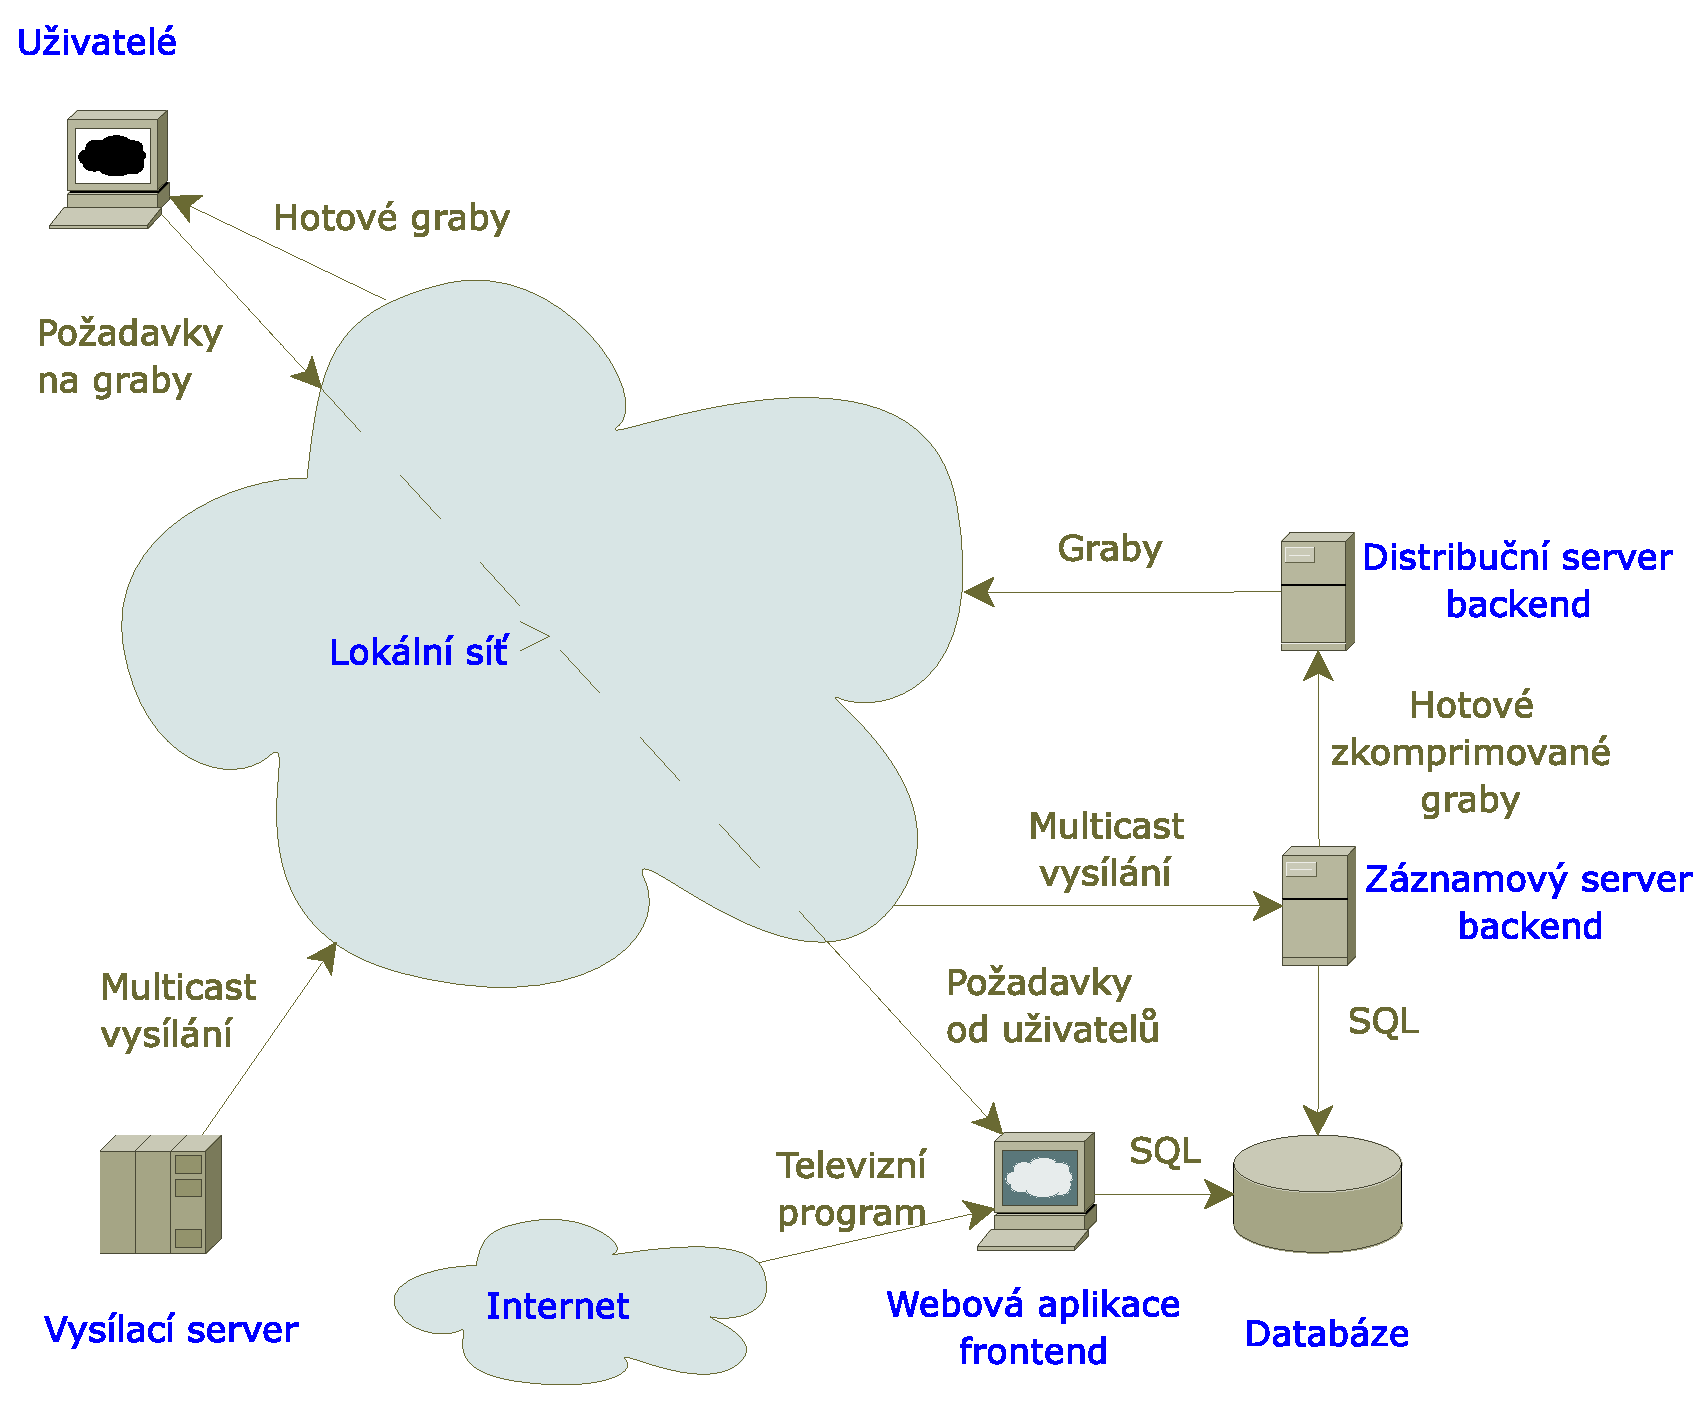
\includegraphics[width=15cm]{images/dvbgrab.eps}
\caption{Systém DVBgrabu}
\label{fig:overview}
\end{center}
\end{figure}

Pro funkci systému potřebujeme audio-video signál přenášený po lokální síti, zdroj televizního programu pro všechny nahrávané TV kanály. Uživatel poté objednává nahrávku (grab) pouhým kliknutím na název pořadu. Hotová nahrávka se komprimuje do uživatelem preferovaného formátu a výsledek je poté připraven ke stažení. O dostupnosti nové nahrávky je uživatel, který si ji objednal, informován e-mailem.
\vfill
\pagebreak
\section{Vlastnosti DVBgrabu}
\bitem
\item Podpora distribuce nahrávek také přes HTTP server apache
\item Webové konfigurační rozhraní setup.php
\item Sjednocená a centralizovaná konfigurace v jednom souboru config.php
\item Možnost volby preferovaného formátu hotové nahrávky (MPEG-2, MPEG-4, ...)
\item Možnost nahrávat z několika kanálů paralelně, odpadá potřeba volit, který z analogových kanálů bude naladěn v době záznamu
\item Záznamové skripty pracující s libovolným audio-video signálem šířeným po lokální síti
\item Využití ADOdb pro abstraktní přístup k téměř libovolnému databázovému stroji
\item Seznam hotových nahrávek ve webovém rozhraní obsahuje i odkazy na stažení
\item Objednávání nahrávek přímo z vyhledávacího formuláře
\item Možnost dodatečných změn nastavení uživatelského účtu, případně zrušení účtu
\item Zasílání nového hesla při zapomenutí starého
\item Kompletní vícejazyčná podpora
\item K dispozici kromě češtiny je také angličtina, francouzština a slovenština
\item Automatický výběr použitého jazyku ve webovém rozhraní
\item Podpora načítání TV programu ve formátu XMLTV
\item Automatická údržba záznamového serveru
\item Podpora zobrazování detailních záznamů až při požadavku pomocí asynchronních XMLHTTP požadavků
\item Detailní informace o pořadu k dispozici společně s nahrávkou ve formátu XML s připojenou XSL transformací.
\eitem

\section{Servery}
Systém využívá ke svému běhu 2 různé servery, i když to není nutností. Na jednom běží databáze a webové rozhraní. Na druhém potom vysílání signálu do lokální sítě, záznam na disk a distribuce nahraných pořadů.
\section{Databáze}
Jako databázový server lze použít téměř libovolnou SQL databázi, protože systém využívá knihovnu ADOdb, která podporuje v současné době zhruba 15 různých databázových strojů. Systém byl provozován na MySQL databázi, nyní na PostgreSQL. Kvůli použití ADOdb je nutné vždy volat SQL kód jen s použitím ADOdb funkcí, například pro formátování datumu v SQL dotazech musí být vždy volána odpovídající ADOdb funkce, která vygeneruje funkci odpovídající aktuálně použitému databázovému serveru.
\section{Webové stránky}
Webové prostředí je napsáno pomocí XHTML+PHP+JavaScript. Obsahuje jak uživatelské tak administrativní rozhraní převážně pro prvotní nastavení a případné změny v konfiguraci. Je napsáno s podporou více jazykových variant (čeština, slovenština, angličtina, francouzština). Všechny zobrazované texty jsou definovány jako konstanty v souborech lang/lang.jazyk.php.

Jazyk se volí postupně podle těchto pravidel:
\bitem
\item podle cookie, pokud uživatel někdy přepnul jazyk ručně kliknutím na ikonu vlajky
\item podle preferovaných jazyků v nastavení prohlížeče
\item v databázi hledáme poslední použitý jazyk daného uživatele
\item výchozí jazyk definovaný v globální konfiguraci 
\eitem

Nakonec se zvolený jazyk uloží do databáze k uživateli jako poslední použitý jazyk. To se využívá například při odesílání e-mailu o úspěšném nahrání, kdy nemáme již k dispozici uživatele, jeho cookies ani jeho prohlížeč.

Z důvodu vícejazyčného webového rozhraní je třeba zajistit také kódování v databázi nastavené na UTF-8, aby podporovala všechny přípustné varianty.

\section{Záznam}

O nahrávání se starají 2 nekonečné smyčky naprogramované také v PHP. Jedna se stará \linebreak[4]o~záznam (grab\_loop), druhá o komprimaci (encode\_loop). Záznamová smyčka se spouští po startu systému a v krátkych časových intervalech kontroluje, zda na některém kanálu nezačíná nějaký objednaný pořad. 
Pokud ano, spustí na pozadí nový proces, který zajistí záznam tohoto pořadu (grab\_process, kterému se předává pouze ID záznamu v databázi) a sama pokračuje dál ve své činnosti.

Komprimační smyčka je odlišná, spouští se sice také po startu systému, ale protože nemá smysl pouštět paralelně příliš mnoho komprimačních procesů, tak vždy kontroluje, zda existuje v~databázi nějaký nevyřízený požadavek na formát, do kterého se zrovna nic nekomprimuje. Pokud ano, vybere nejstarší podle data vysílání pořadu a spustí nový proces (encode\_process, kterému předává ID požadavku a formát, jaký se má použít). To znamená, že kolik různých formátů si uložíme do databázové tabulky encoder, tolik komprimačních procesů může běžet paralelně.

Vlastní záznam na disk je prováděn pomocí programu dumprtp, z balíku dvbstream, který ukládá datový tok ze zadané IP adresy a portu do souboru. V záznamovém procesu se nejdříve všechny požadavky na daný pořad přepnou ze stavu \quotedblbase naplánován'' do stavu \quotedblbase ukládá se''. Poté je dumprtp spouštěn jako volání podprocesu na pozadí a poté je počítán čas až do konce pořadu, kdy se pošle procesu dumprtp signál TERM k ukončení. 

Data se při ukládání netransformují, takže zůstanou uložena jako MPEG-TS (transport stream). To umožňuje paralelní zápis několika pořadů na disk, protože je to operace relativně nenáročná. Transport stream je optimalizovaný spíše pro přenos audio-video signálů, než pro jejich přehrávání (neobsahuje příliš často klíčové snímky, takže například při posunech je dlouhá odezva než se obnoví obraz). Z jaké IP adresy a portu se má ukládat, je nyní určeno v databázi v definici televizního kanálu.

Jmenné konvence pro název nahrávky jsou DVB- jako předpona, pak datum ve formátu Ymd-Hi (rok, měsíc, den, hodiny, minuty) tak, aby se adresář s nahrávkami dal řadit chronologicky podle abecedy. Dále následuje jméno kanálu (po odstranění diakritiky) a název pořadu, buď po odstranění diakritiky nebo jenom ID záznamu, pokud to je v konfiguraci nastaveno (přesné jméno pořadu včetně diakritiky je pak až v popisném XML souboru, viz dále. Nekomprimované nahrávky mají příponu .ts jako transport stream.

Po ukončení dumprtp smyčka ještě zkontroluje, zda má nahrávka nějakou odpovídající nenulovou velikost a informace o uložení se aktualizuje v databázi (všechny požadavky na tento pořad přejdou ze stavu \quotedblbase ukládá se'' do stavu \quotedblbase uložen''.

\section{Specifika ukládání z digitálního vysílání}
Součástí DVB vysílání jsou i informace o vysílaných pořadech.

Tyto informace jsou vysílány jako součást MPEG-2 dat pomocí protokolu PMCP (Programming Metadata Communication Protocol), což jsou do XML balené data z PSIP (Program and System Information Protocol).

Součástí PSIP jsou následující tabulky:
\bitem
\item \textbf{STT} (system time table) -- aktuální čas vysílaný každou sekundu
\item \textbf{MGT} (master guide table) -- datové ukazatale do dalších tabulek PSIP
\item \textbf{VCT} (virtual channel table) -- seznam kanálů a přiřazení jejich čísel
\item \textbf{RRT} (rating region table) -- hodnocení obsahu pro jednotlivé regiony
\item \textbf{EIT} (event information table) -- názvy a další data pro televizní program
\item \textbf{ETT} (extended text table) -- detailní popis programů
\item \textbf{DCCT} (directed channel change table)
\item \textbf{DCCST} (directed channel change selection code table)
\eitem

Tabulky EIT a ETT používá v MHP (Multimedia Home Platform -- aplikační rozšíření v DVB) aplikace EPG (Electronic program guide -- elektronický televizní program). Tyto informace by bylo velmi výhodné použít pro přesné nastavení začátku a konce záznamu.

Pokud toto nemáme k dispozici, musí nahrávání začínat několik minut před plánovaným začátkem pořadu (lze konfigurovat kolik) a také lze nastavit, kolik minut se má nahrávat po plánovaném konci pořadu.

Pokud bychom chtěli využít informace z EIT přímo v DVBgrabu, tak bychom museli nejdříve zajistit jejich distribuci z vysílajícího serveru do lokální sítě.

Podle zástupců Czech Digital Group jsou prý tyto údaje již dostupné. Pokud jim televize údaje dodá, tak je pouze převedou do formátu vhodného pro EIT a vloží do toku dat.

Pokud by v EIT byly obsaženy i značky začátku a konce televizní reklamy, tak by šlo podle nich vypínat a zapínat záznam, a tím tedy zajistit automatické vystřihování reklamy. Případně by bylo možné naprogramovat nějaký vlastní algoritmus pro poznávání reklamy (třeba podle podobnosti s dodanou počáteční a koncovou znělkou). Tento algoritmus by byl pravděpodobně dosti hardwarově náročný, což by při několika paralelních záznamech mohlo vést až ke ztrátám snímku, proto nebyl použit. Tyto algoritmy také nemusí být v souladu se zákonem (automatický systém na vystřihování reklamy byl součástí software DVD rekordérů KISS a~musel být odstraněn a~zůstalo pouze automatické přetáčení reklamy při sledování ze záznamu).
\vfill
\pagebreak
\section{Komprimace záznamů}
Komprimační smyčka postupně prochází přes všechny formáty (encodery) a zkoumá, zda pro ty, které aktuálně neběží (nemají v databázi uložené své číslo procesu PID, pokud je uloženo, tak se testuje, zda doopravdy běží), neexistuje nějaký čekající požadavek ve stavu \quotedblbase uložen''. Pokud ano, vybere opět nejstarší. Založí na pozadí nový proces, který komprimaci zajistí. Komprimační proces nejdříve opět změní stav požadavku~v databázi z \quotedblbase uložen'' na \quotedblbase komprimuje se''.
 
Poté spustí skript, jehož jméno je opět uvedeno v~databázi a který musí být uložen v adresáři encoders. Tomuto skriptu předá název nahraného pořadu, který do databáze uložil předcházející záznamový proces, a z původního jména vytvoří název cílového souboru připojením definované přípony z databáze. Po úspěšné komprimaci je z .ts souboru vytvořen například .avi soubor ve formátu MPEG-4, poté se znovu zkontroluje, zda výsledný soubor má odpovídající velikost, a~pokud ano, dojde k uveřejnění nahrávky požadujícím uživatelům. 

\section{Komprimační formáty}
Komprimaci zajišťuje program mencoder, který podporuje velmi mnoho formátů. Některé základní jsem uvedl v příloze.
Čím více kombinací kontejner, video, audio kodeků umožníme uživateli zvolit, tím větší budou nároky na čas a místo na disku. Každá nahrávka totiž musí být zkomprimována do všech uživateli požadovaných variant a také bude ve všech požadovaných variantách uložena na vyhrazeném diskovém prostoru.

Proto je připraveno pouze pár zajímavých kombinací, a to:

\bitem
\item \textbf{MPEG-2 TS} -- formát v jakém přijímáme DVB signál ze sítě, soubor bude mít příponu .mpg.
\item \textbf{AVI/MPEG-4 ASP (z libavcodec)/MP3} -- běžně používaný komprimovaný soubor, hodina záznamu odpovídá zhruba 700MB. Jsou předdefinované varianty s různým měřítkem (různé rozlišení), soubor bude mít příponu .avi.
\eitem
Dále by bylo vhodné použít:
\bitem
\item \textbf{OGG/Theora/Vorbis} -- svobodná obdoba předchozí kombinace s mírně efektivnějším poměrem kvality a velikosti souboru, s příponou .ogg.
\item \textbf{MP4/MPEG-4 AVC (z x264)/AAC} -- nejvyšší kvalita, pokud budeme mít dostatečně kvalitní zdroj, přípona by byla .mp4. Tato varianta bude trvat mnohem déle, proto je vhodná jen pro výkonnější servery nebo tam, kde nevadí časový rozdíl mezi koncem pořadu a uveřejněním grabu.
\eitem
\section{Uveřejnění nahrávky}
\subsection{Popisný XML soubor}
Je vytvářen XML soubor popisující detaily nahrávky. Obsahuje název pořadu s diakritikou, název kanálu s diakritikou, začátek a konec pořadu podle televizního programu, začátek a konec nahrávání, použitý komprimační formát, výslednou velikost souboru v kB a MD5 součet pro kontrolu bezchybného stažení.

XML soubor je ve webovém prohlížeči zobrazován v podobě přehledné tabulky, která je z XML souboru vytvořena podle XSL šablony.

Ta je v uživatelském adresáři vygenerována (podle jazyku, který uživatel používá na webovém rozhraní DVBgrabu) v souboru dvbgrab.xsl. Pokud uživatel chce stejně zobrazovat i stažené XML soubory, musí k nim do adresáře zkopírovat i tento soubor.

\subsection{Vytvoření symbolického odkazu}
Vytvoření symbolického odkazu z uživatelova adresáře do sdíleného prostoru, ve kterém jsou uložené všechny nahrávky (jak na nahrávku, tak na odpovídající XML soubor).

\subsection{Kontrola a případné založení uživatelského adresáře}
Během vytváření symbolických odkazů dojde také ke kontrole, zda je uživatelský adresář již založen a případně také k přegenerování souboru .htaccess, který určuje ze kterých IP adres smí uživatel své nahrávky stahovat (tato IP adresa je vždy pouze jedna a je uložena v databázi u~informací o uživateli). Uživatel má možnost přes webové rozhraní zadat její změnu, proto musí docházet k přegenerování těchto .htaccess souborů. Druhá varianta je přegenerování souboru pouze pokud nějaká změna skutečně nastala, což rozhoduje údržbový skript pouštěný pomocí plánovače cron. 

Oba přístupy mají své výhody, ale i nevýhody. První je nevýhodný například pro uživatele, který při pokusu o stažení nahrávky zjistí, že má zaregistrovanou neaktuální IP a další nahrávku zatím neplánuje. Druhý naopak nepotěší uživatele, který ráno zadá změnu IP, v poledne se mu uloží nahrávka a až do půlnoci nejde stáhnout, když se údržbové skripty budou pouštět jen 1x denně o půlnoci. Řešením je buď dostatečně časté pouštění údržby nebo kombinace obou přístupů. Výchozí nastavení generuje .htaccess soubory v obou případech.

\subsection{Odeslání e-mailu a označení v databázi}
Odeslání informačního e-mailu všem uživatelům, kteří tuto nahrávku v tomto formátu požadovali. U všech uživatelských požadavků je v databázi nastaveno jméno souboru s nahrávkou, jak bude přístupná přes http server, což je pak použito pro generování odkazů na stažení v sekci \quotedblbase moje graby''.

\section{Distribuce záznamů}
Distribuce nahrávek mezi uživatele je zajištěna přes http server apache (nyní ve verzi 2.2.x, která již nemá problémy se soubory většími než 2GB). Alternativně lze použít i nějaký ftp server, který umí autentifikovat uživatele nejlépe proti použité databázi. Pokud potřebujeme generovat uživatelské účty pro ftp server, máme k dispozici pouze uživatelská jména a md5 součty jejich hesel (musíme číst i md5 hesel z externí autorizační databáze).

\section{Získávání aktuálního televizního programu pro web}
Stahování aktuálního TV programu je zajištěno přes různé moduly. V adresáři tvgrabbers jsou jednotlivé php skripty. V distribuci je skript tv\_grab\_novinky\_cz/tv\_grab\_novinky\_cz.php, který načítá data ze serveru novinky.cz. Stažený html kód je zpracován pomocí regulárních výrazů a jednotlivé pořady jsou uloženy do databáze. Tento skript umí pouze několik programů (ČT1, ČT2, Nova, Prima), pro načítání jiných je nutné skript editovat.

XMLTV -- dalším skriptem v distribuci je xmltv\_to\_db.php, který lze použít pro vkládání XML souboru ve formátu XMLTV do databázové tabulky television. Nejdříve se podíváme, co je to XMLTV. XMLTV je specifikace, jak zapisovat televizní program do XML souborů. Tuto specifikaci využívá velmi mnoho programů viz. \cite{xmltvURL}. Na stránkách XMLTV lze stáhnout též instalační balík, který obsahuje stahovací skripty pro poměrně mnoho zemí. Bohužel není obsažen skript po Českou republiku z důvodu, který uvedu v následující sekci.

Každý stahovací skript musí být před prvním použitím spuštěn v konfiguračním řežimu (např. pro skript tv\_grab\_cz takto \quotedblbase tv\_grab\_cz -conf''). Konfigurace se obvykle skládá z několika obecných dotazů. Dále se vypisuje seznam televizních kanálů, které umí stahovat, a pro každý kanál uživatel volí, zda se má stahovat, či ne. Poté stačí spustit skript s parametrem udávajícím na kolik dnů dopředu má stahovat, případně od kolikáteho dne začít (\quotedblbase tv\_grab\_cz --days 10'', stáhne na 10 dní dopředu pro všechny povolené kanály jejich program). Výstupem skriptu je správně formátovaný soubor XML, který ještě potřebujeme transformovat do databáze.

Protože se nám hodí i koncové časy pořadů, pomůže nám pomocný skript z balíku XMLTV tv\_sort, který nejen chronologicky seřadí pořady v rámci kanálu, ale také každý pořad doplní koncovým časem (podle počátečního času chronologicky následujícího pořadu). Bohužel tohle selhává u posledních pořadů v rámci dne, kdy následujícím pořadem je až první ranní pořad dalšího dne. Tyto situace se snaží detekovat systém až při vytváření požadavku na nahrání a~pokud pořad začíná mezi 1. a 5. hodinou ranní a trvá déle než 4 hodiny, tak se koncový čas nastaví jen na čas počáteční + definovaná konstanta (výchozí hodnota je +2 hodiny). Pokud koncové časy nemáme v databázi vůbec (např. po použití modulu tv\_grab\_novinky\_cz.php), tak se koncový čas určuje také při vytváření požadavku na nahrání.

Takto předzpracovaný program již můžeme zpracovávat pomocí skriptu xmltv\_to\_db.php. Ten složí pro každý element <programme> 2 SELECT dotazy, INSERT pro vložení a UPDATE pro aktualizaci. První dotaz zjistí, zda v danou dobu na daném kanálu již existuje v databázi pořad se stejným jménem, a pokud ano, element je ignorován. Jinak se provede druhý dotaz, který zjišťuje, zda neexistuje v tu dobu pořad s jiným jménem. Pokud ano, použije se vygenerovaný UPDATE, pokud ne, použije se INSERT. Pokud se ve vstupním souboru objeví například pořad na kanálu, jehož xmltv id nemáme v databázi DVBgrabu registrováno, vypíše se varování a pořad se také nevkládá.

\section{Právní aspekty získávání televizního programu z veřejně dostupných webových stránek}
V zahraničí je běžné, že dostupnost XMLTV formátu programu je částečně podporovaná i~státem. 

U nás tomu bohužel tak není a kvůli tomu v XMLTV distribuci stahovací skript pro Českou republiku v dohledné době asi nenajdeme. Dokonce tam jistou dobu byl již i obsažen. Bohužel firma provozující servery, které sloužily jako zdroj programu pro jinou firmu, která zajišťovala transformaci z HTML formátu do XMLTV, nebyla této aktivitě příznivě nakloněna, a tak byl projekt českého XMLTV pod hrozbou žaloby zastaven.

Bohužel i mně jako tvůrci DVBgrabu byla zaslána žádost o urychlené odstranění načítání televizního programu ze stránek http://www.ceskenoviny.cz, jejichž provozovatelem je Česká tisková kancelář (ČTK), jinak by záležitost řešilo právní oddělení ČTK. Proto nová verze DVBgrabu bude distribuována bez českého XMLTV modulu. Správce systému je pak nucen použít skript tv\_grab\_novinky\_cz.php (za předpokladu, že snad přátelštější provozovatel http://www.seznam.cz nepřijde s žádostí o odstranění) a nebo si zajistit xmltv zdroj svépomocí.

Doufejme, že si některý portál nabízející online TV program v HTML podobě co nejdříve všimne na trhu tohoto nedostatku a doplní své portfolio služeb například o placený přístup k XMLTV formátu svého programu.
\vfill
